\documentclass[border=10pt]{standalone}
\usepackage{tikz}
\usetikzlibrary{calc}

\begin{document}
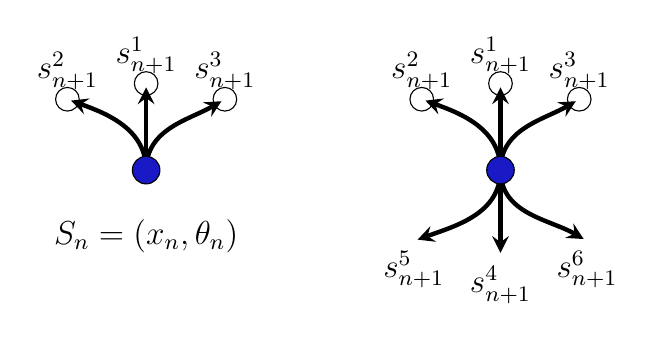
\begin{tikzpicture}[
    text=black,
    >={stealth},
    dot/.style={circle, fill=black!25!blue!90, draw=black, minimum size=3.5mm, inner sep=0pt},
    hollowcircle/.style={circle, draw=black, fill=white, minimum size=3mm, inner sep=0pt},
    arrowline/.style={->, shorten >=0.5mm},
]

% ==================== LEFT DIAGRAM ====================
\begin{scope}[shift={(-2,0)}]
    % Text label (Now moved to the bottom as in the original)
    \node[anchor=north] at (0,-0.5) {\large $S_n = (x_n, \theta_n)$};

    \coordinate (L_center) at (0, 0);

    % Top hollow circles
    \node[hollowcircle] (L_left) at (-1,0.9) {};
    \node[hollowcircle] (L_mid)  at (0,1.1) {};
    \node[hollowcircle] (L_right) at (1,0.9) {};

    % Arched lines from the blue dot TO hollow circles
    \draw[arrowline, ->, ultra thick] (L_center) to[out=90, in=-20] (L_left.center);
    \draw[arrowline, ->, ultra thick] (L_center) to[out=90, in=-90] (L_mid.center);
    \draw[arrowline, ->, ultra thick] (L_center) to[out=90, in=210] (L_right.center);

        % Central blue dot
    \node[dot] (L_center) at (0,0) {};

    % Top labels
    \node[anchor=south] at (L_left) {\large $s_{n+1}^2$};
    \node[anchor=south] at (L_mid)  {\large $s_{n+1}^1$};
    \node[anchor=south] at (L_right) {\large $s_{n+1}^3$};    
\end{scope}

% ==================== RIGHT DIAGRAM ====================
\begin{scope}[shift={(2.5,0)}] % Shift to the right

    \coordinate (R_center) at (0, 0);

    % Top hollow circles
    \node[hollowcircle] (R_t_left) at (-1,0.9) {};
    \node[hollowcircle] (R_t_mid)  at (0,1.1) {};
    \node[hollowcircle] (R_t_right) at (1,0.9) {};

    % Arched lines TO top hollow circles
    \draw[arrowline, ->, ultra thick] (R_center) to[out=90, in=-20] (R_t_left.center);
    \draw[arrowline, ->, ultra thick] (R_center) to[out=90, in=-90] (R_t_mid.center);
    \draw[arrowline, ->, ultra thick] (R_center) to[out=90, in=210] (R_t_right.center);

    % Top labels
    \node[anchor=south] at (R_t_left) {\large $s_{n+1}^2$};
    \node[anchor=south] at (R_t_mid)  {\large $s_{n+1}^1$};
    \node[anchor=south] at (R_t_right) {\large $s_{n+1}^3$};

    % Bottom endpoints for arrows (adjusted positions for correct arrow direction)
    \coordinate (R_b_left) at (-1.1,-0.9);
    \coordinate (R_b_mid)  at (0,-1.1);
    \coordinate (R_b_right) at (1.1,-0.9);

    % Straight lines FROM the center to bottom positions
    \draw[arrowline, ->, ultra thick] (R_center) to[out=-90, in=20] (R_b_left);
    \draw[arrowline, ->, ultra thick] (R_center) to[out=-90, in=90] (R_b_mid);
    \draw[arrowline, ->, ultra thick] (R_center) to[out=-90, in=-210] (R_b_right);

        % Central blue dot
    \node[dot] (R_center) at (0,0) {};

    % Bottom labels
    \node[anchor=north] at (R_b_left) {\large $s_{n+1}^5$};
    \node[anchor=north] at (R_b_mid)  {\large $s_{n+1}^4$};
    \node[anchor=north] at (R_b_right) {\large $s_{n+1}^6$};
\end{scope}

\end{tikzpicture}
\end{document}